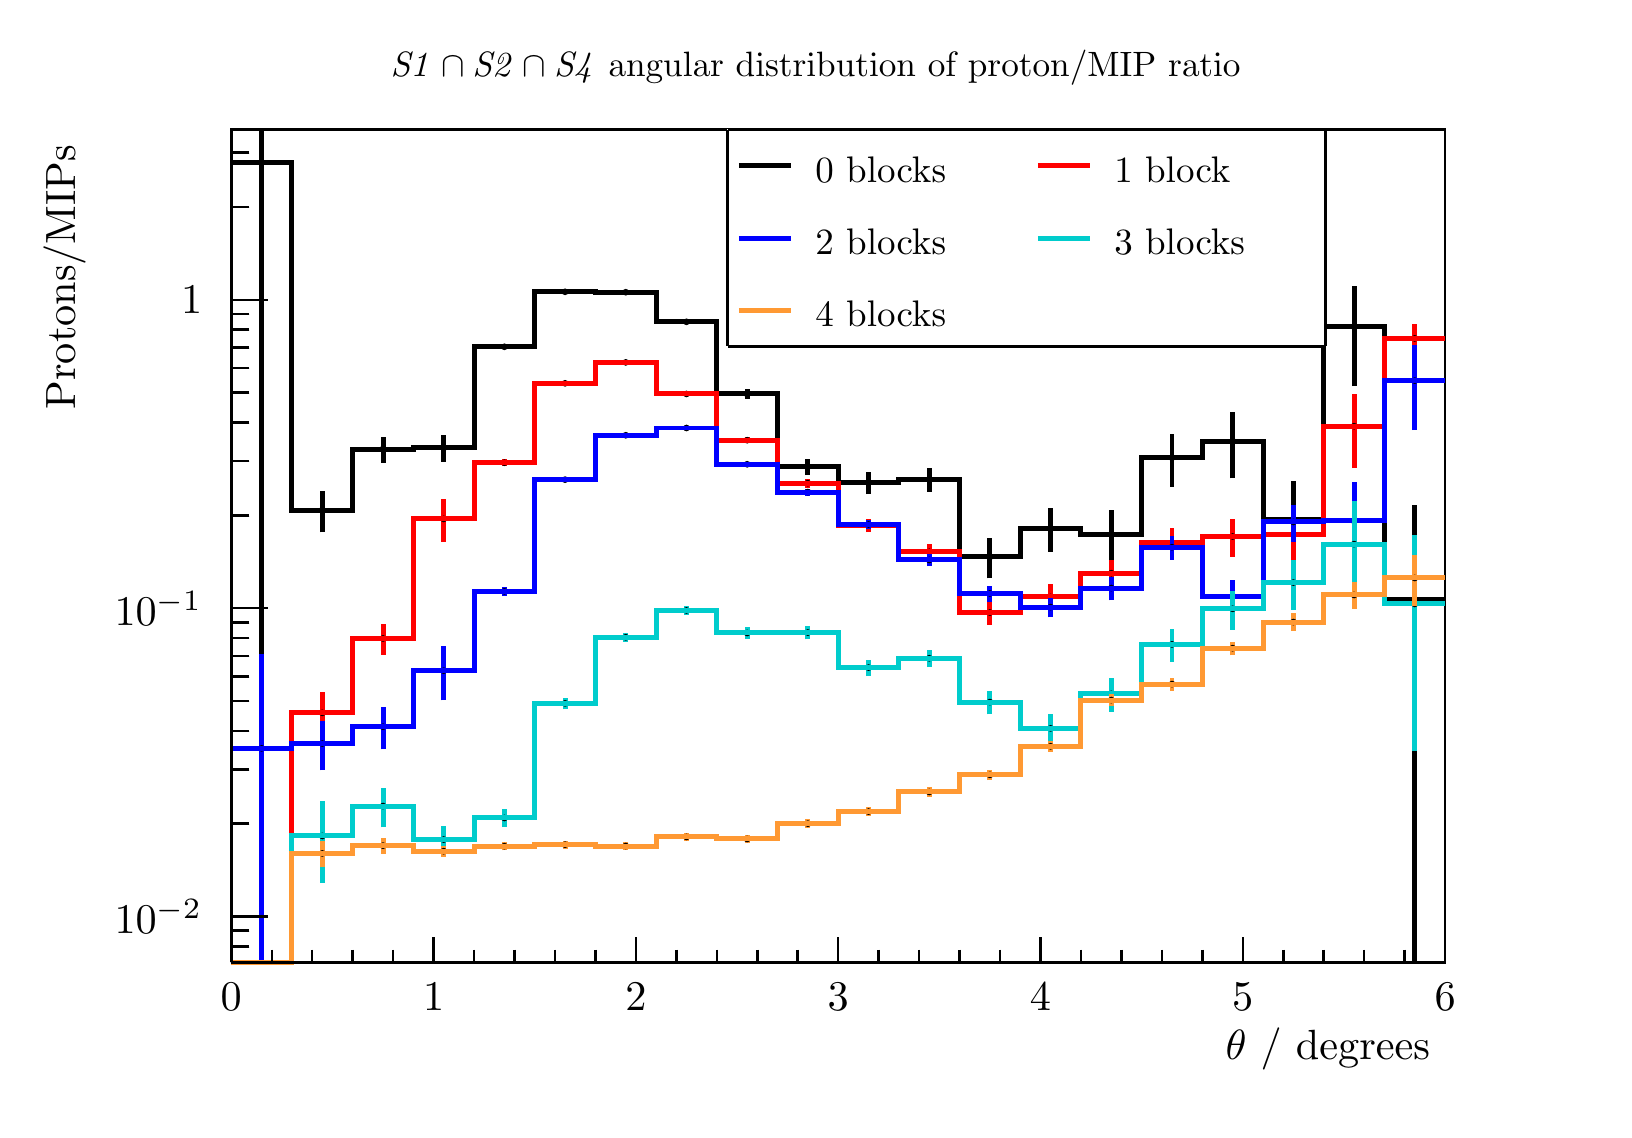
\begin{tikzpicture}
\pgfdeclareplotmark{cross} {
\pgfpathmoveto{\pgfpoint{-0.3\pgfplotmarksize}{\pgfplotmarksize}}
\pgfpathlineto{\pgfpoint{+0.3\pgfplotmarksize}{\pgfplotmarksize}}
\pgfpathlineto{\pgfpoint{+0.3\pgfplotmarksize}{0.3\pgfplotmarksize}}
\pgfpathlineto{\pgfpoint{+1\pgfplotmarksize}{0.3\pgfplotmarksize}}
\pgfpathlineto{\pgfpoint{+1\pgfplotmarksize}{-0.3\pgfplotmarksize}}
\pgfpathlineto{\pgfpoint{+0.3\pgfplotmarksize}{-0.3\pgfplotmarksize}}
\pgfpathlineto{\pgfpoint{+0.3\pgfplotmarksize}{-1.\pgfplotmarksize}}
\pgfpathlineto{\pgfpoint{-0.3\pgfplotmarksize}{-1.\pgfplotmarksize}}
\pgfpathlineto{\pgfpoint{-0.3\pgfplotmarksize}{-0.3\pgfplotmarksize}}
\pgfpathlineto{\pgfpoint{-1.\pgfplotmarksize}{-0.3\pgfplotmarksize}}
\pgfpathlineto{\pgfpoint{-1.\pgfplotmarksize}{0.3\pgfplotmarksize}}
\pgfpathlineto{\pgfpoint{-0.3\pgfplotmarksize}{0.3\pgfplotmarksize}}
\pgfpathclose
\pgfusepathqstroke
}
\pgfdeclareplotmark{cross*} {
\pgfpathmoveto{\pgfpoint{-0.3\pgfplotmarksize}{\pgfplotmarksize}}
\pgfpathlineto{\pgfpoint{+0.3\pgfplotmarksize}{\pgfplotmarksize}}
\pgfpathlineto{\pgfpoint{+0.3\pgfplotmarksize}{0.3\pgfplotmarksize}}
\pgfpathlineto{\pgfpoint{+1\pgfplotmarksize}{0.3\pgfplotmarksize}}
\pgfpathlineto{\pgfpoint{+1\pgfplotmarksize}{-0.3\pgfplotmarksize}}
\pgfpathlineto{\pgfpoint{+0.3\pgfplotmarksize}{-0.3\pgfplotmarksize}}
\pgfpathlineto{\pgfpoint{+0.3\pgfplotmarksize}{-1.\pgfplotmarksize}}
\pgfpathlineto{\pgfpoint{-0.3\pgfplotmarksize}{-1.\pgfplotmarksize}}
\pgfpathlineto{\pgfpoint{-0.3\pgfplotmarksize}{-0.3\pgfplotmarksize}}
\pgfpathlineto{\pgfpoint{-1.\pgfplotmarksize}{-0.3\pgfplotmarksize}}
\pgfpathlineto{\pgfpoint{-1.\pgfplotmarksize}{0.3\pgfplotmarksize}}
\pgfpathlineto{\pgfpoint{-0.3\pgfplotmarksize}{0.3\pgfplotmarksize}}
\pgfpathclose
\pgfusepathqfillstroke
}
\pgfdeclareplotmark{newstar} {
\pgfpathmoveto{\pgfqpoint{0pt}{\pgfplotmarksize}}
\pgfpathlineto{\pgfqpointpolar{44}{0.5\pgfplotmarksize}}
\pgfpathlineto{\pgfqpointpolar{18}{\pgfplotmarksize}}
\pgfpathlineto{\pgfqpointpolar{-20}{0.5\pgfplotmarksize}}
\pgfpathlineto{\pgfqpointpolar{-54}{\pgfplotmarksize}}
\pgfpathlineto{\pgfqpointpolar{-90}{0.5\pgfplotmarksize}}
\pgfpathlineto{\pgfqpointpolar{234}{\pgfplotmarksize}}
\pgfpathlineto{\pgfqpointpolar{198}{0.5\pgfplotmarksize}}
\pgfpathlineto{\pgfqpointpolar{162}{\pgfplotmarksize}}
\pgfpathlineto{\pgfqpointpolar{134}{0.5\pgfplotmarksize}}
\pgfpathclose
\pgfusepathqstroke
}
\pgfdeclareplotmark{newstar*} {
\pgfpathmoveto{\pgfqpoint{0pt}{\pgfplotmarksize}}
\pgfpathlineto{\pgfqpointpolar{44}{0.5\pgfplotmarksize}}
\pgfpathlineto{\pgfqpointpolar{18}{\pgfplotmarksize}}
\pgfpathlineto{\pgfqpointpolar{-20}{0.5\pgfplotmarksize}}
\pgfpathlineto{\pgfqpointpolar{-54}{\pgfplotmarksize}}
\pgfpathlineto{\pgfqpointpolar{-90}{0.5\pgfplotmarksize}}
\pgfpathlineto{\pgfqpointpolar{234}{\pgfplotmarksize}}
\pgfpathlineto{\pgfqpointpolar{198}{0.5\pgfplotmarksize}}
\pgfpathlineto{\pgfqpointpolar{162}{\pgfplotmarksize}}
\pgfpathlineto{\pgfqpointpolar{134}{0.5\pgfplotmarksize}}
\pgfpathclose
\pgfusepathqfillstroke
}
\definecolor{c}{rgb}{1,1,1};
\draw [color=c, fill=c] (0,0) rectangle (20,13.7249);
\draw [color=c, fill=c] (2.5788,1.86246) rectangle (17.9943,12.4355);
\definecolor{c}{rgb}{0,0,0};
\draw [c,line width=0.9] (2.5788,1.86246) -- (2.5788,12.4355) -- (17.9943,12.4355) -- (17.9943,1.86246) -- (2.5788,1.86246);
\definecolor{c}{rgb}{1,1,1};
\draw [color=c, fill=c] (2.5788,1.86246) rectangle (17.9943,12.4355);
\definecolor{c}{rgb}{0,0,0};
\draw [c,line width=0.9] (2.5788,1.86246) -- (2.5788,12.4355) -- (17.9943,12.4355) -- (17.9943,1.86246) -- (2.5788,1.86246);
\definecolor{c}{rgb}{0,0,0.6};
\draw [c,line width=0.9] (2.5788,1.86246) -- (3.34957,1.86246) -- (3.34957,1.86246) -- (4.12034,1.86246) -- (4.12034,1.86246) -- (4.89112,1.86246) -- (4.89112,1.86246) -- (5.66189,1.86246) -- (5.66189,1.86246) -- (6.43266,1.86246) --
 (6.43266,1.86246) -- (7.20344,1.86246) -- (7.20344,1.86246) -- (7.97421,1.86246) -- (7.97421,1.86246) -- (8.74499,1.86246) -- (8.74499,1.86246) -- (9.51576,1.86246) -- (9.51576,1.86246) -- (10.2865,1.86246) -- (10.2865,1.86246) -- (11.0573,1.86246)
 -- (11.0573,1.86246) -- (11.8281,1.86246) -- (11.8281,1.86246) -- (12.5989,1.86246) -- (12.5989,1.86246) -- (13.3696,1.86246) -- (13.3696,1.86246) -- (14.1404,1.86246) -- (14.1404,1.86246) -- (14.9112,1.86246) -- (14.9112,1.86246) --
 (15.6819,1.86246) -- (15.6819,1.86246) -- (16.4527,1.86246) -- (16.4527,1.86246) -- (17.2235,1.86246) -- (17.2235,1.86246) -- (17.9943,1.86246);
\definecolor{c}{rgb}{0,0,0};
\draw [c,line width=0.9] (2.5788,1.86246) -- (17.9943,1.86246);
\draw [c,line width=0.9] (2.5788,2.17983) -- (2.5788,1.86246);
\draw [c,line width=0.9] (3.09265,2.02115) -- (3.09265,1.86246);
\draw [c,line width=0.9] (3.60649,2.02115) -- (3.60649,1.86246);
\draw [c,line width=0.9] (4.12034,2.02115) -- (4.12034,1.86246);
\draw [c,line width=0.9] (4.63419,2.02115) -- (4.63419,1.86246);
\draw [c,line width=0.9] (5.14804,2.17983) -- (5.14804,1.86246);
\draw [c,line width=0.9] (5.66189,2.02115) -- (5.66189,1.86246);
\draw [c,line width=0.9] (6.17574,2.02115) -- (6.17574,1.86246);
\draw [c,line width=0.9] (6.68959,2.02115) -- (6.68959,1.86246);
\draw [c,line width=0.9] (7.20344,2.02115) -- (7.20344,1.86246);
\draw [c,line width=0.9] (7.71729,2.17983) -- (7.71729,1.86246);
\draw [c,line width=0.9] (8.23114,2.02115) -- (8.23114,1.86246);
\draw [c,line width=0.9] (8.74499,2.02115) -- (8.74499,1.86246);
\draw [c,line width=0.9] (9.25883,2.02115) -- (9.25883,1.86246);
\draw [c,line width=0.9] (9.77268,2.02115) -- (9.77268,1.86246);
\draw [c,line width=0.9] (10.2865,2.17983) -- (10.2865,1.86246);
\draw [c,line width=0.9] (10.8004,2.02115) -- (10.8004,1.86246);
\draw [c,line width=0.9] (11.3142,2.02115) -- (11.3142,1.86246);
\draw [c,line width=0.9] (11.8281,2.02115) -- (11.8281,1.86246);
\draw [c,line width=0.9] (12.3419,2.02115) -- (12.3419,1.86246);
\draw [c,line width=0.9] (12.8558,2.17983) -- (12.8558,1.86246);
\draw [c,line width=0.9] (13.3696,2.02115) -- (13.3696,1.86246);
\draw [c,line width=0.9] (13.8835,2.02115) -- (13.8835,1.86246);
\draw [c,line width=0.9] (14.3973,2.02115) -- (14.3973,1.86246);
\draw [c,line width=0.9] (14.9112,2.02115) -- (14.9112,1.86246);
\draw [c,line width=0.9] (15.425,2.17983) -- (15.425,1.86246);
\draw [c,line width=0.9] (15.9389,2.02115) -- (15.9389,1.86246);
\draw [c,line width=0.9] (16.4527,2.02115) -- (16.4527,1.86246);
\draw [c,line width=0.9] (16.9666,2.02115) -- (16.9666,1.86246);
\draw [c,line width=0.9] (17.4804,2.02115) -- (17.4804,1.86246);
\draw [c,line width=0.9] (17.9943,2.17983) -- (17.9943,1.86246);
\draw [anchor=base] (2.5788,1.24484) node[scale=1.52731, color=c, rotate=0]{0};
\draw [anchor=base] (5.14804,1.24484) node[scale=1.52731, color=c, rotate=0]{1};
\draw [anchor=base] (7.71729,1.24484) node[scale=1.52731, color=c, rotate=0]{2};
\draw [anchor=base] (10.2865,1.24484) node[scale=1.52731, color=c, rotate=0]{3};
\draw [anchor=base] (12.8558,1.24484) node[scale=1.52731, color=c, rotate=0]{4};
\draw [anchor=base] (15.425,1.24484) node[scale=1.52731, color=c, rotate=0]{5};
\draw [anchor=base] (17.9943,1.24484) node[scale=1.52731, color=c, rotate=0]{6};
\draw [anchor= east] (17.9943,0.76447) node[scale=1.52731, color=c, rotate=0]{$\theta$ / degrees};
\draw [c,line width=0.9] (2.5788,1.86246) -- (2.5788,12.4355);
\draw [c,line width=0.9] (2.8099,2.06354) -- (2.5788,2.06354);
\draw [c,line width=0.9] (2.8099,2.26388) -- (2.5788,2.26388);
\draw [c,line width=0.9] (3.04101,2.44309) -- (2.5788,2.44309);
\draw [anchor= east] (2.3988,2.44309) node[scale=1.52731, color=c, rotate=0]{$10^{-2}$};
\draw [c,line width=0.9] (2.8099,3.6221) -- (2.5788,3.6221);
\draw [c,line width=0.9] (2.8099,4.31178) -- (2.5788,4.31178);
\draw [c,line width=0.9] (2.8099,4.80111) -- (2.5788,4.80111);
\draw [c,line width=0.9] (2.8099,5.18066) -- (2.5788,5.18066);
\draw [c,line width=0.9] (2.8099,5.49078) -- (2.5788,5.49078);
\draw [c,line width=0.9] (2.8099,5.75299) -- (2.5788,5.75299);
\draw [c,line width=0.9] (2.8099,5.98011) -- (2.5788,5.98011);
\draw [c,line width=0.9] (2.8099,6.18046) -- (2.5788,6.18046);
\draw [c,line width=0.9] (3.04101,6.35967) -- (2.5788,6.35967);
\draw [anchor= east] (2.3988,6.35967) node[scale=1.52731, color=c, rotate=0]{$10^{-1}$};
\draw [c,line width=0.9] (2.8099,7.53868) -- (2.5788,7.53868);
\draw [c,line width=0.9] (2.8099,8.22835) -- (2.5788,8.22835);
\draw [c,line width=0.9] (2.8099,8.71768) -- (2.5788,8.71768);
\draw [c,line width=0.9] (2.8099,9.09724) -- (2.5788,9.09724);
\draw [c,line width=0.9] (2.8099,9.40736) -- (2.5788,9.40736);
\draw [c,line width=0.9] (2.8099,9.66956) -- (2.5788,9.66956);
\draw [c,line width=0.9] (2.8099,9.89669) -- (2.5788,9.89669);
\draw [c,line width=0.9] (2.8099,10.097) -- (2.5788,10.097);
\draw [c,line width=0.9] (3.04101,10.2762) -- (2.5788,10.2762);
\draw [anchor= east] (2.3988,10.2762) node[scale=1.52731, color=c, rotate=0]{1};
\draw [c,line width=0.9] (2.8099,11.4553) -- (2.5788,11.4553);
\draw [c,line width=0.9] (2.8099,12.1449) -- (2.5788,12.1449);
\draw [anchor= east] (0.461318,12.4355) node[scale=1.52731, color=c, rotate=90]{ Protons/MIPs};
\draw [c,line width=1.8] (2.96418,1.86246) -- (2.96418,12.0197);
\draw [c,line width=1.8] (2.96418,12.0197) -- (2.96418,12.4355);
\foreach \P in {(2.96418,12.0197)}{\draw[mark options={color=c,fill=c},mark size=2.402402pt,mark=*,mark size=1pt] plot coordinates {\P};}
\draw [c,line width=1.8] (3.73496,7.32116) -- (3.73496,7.60568);
\draw [c,line width=1.8] (3.73496,7.60568) -- (3.73496,7.84935);
\foreach \P in {(3.73496,7.60568)}{\draw[mark options={color=c,fill=c},mark size=2.402402pt,mark=*,mark size=1pt] plot coordinates {\P};}
\draw [c,line width=1.8] (4.50573,8.20864) -- (4.50573,8.38079);
\draw [c,line width=1.8] (4.50573,8.38079) -- (4.50573,8.53711);
\foreach \P in {(4.50573,8.38079)}{\draw[mark options={color=c,fill=c},mark size=2.402402pt,mark=*,mark size=1pt] plot coordinates {\P};}
\draw [c,line width=1.8] (5.2765,8.22) -- (5.2765,8.39484);
\draw [c,line width=1.8] (5.2765,8.39484) -- (5.2765,8.55337);
\foreach \P in {(5.2765,8.39484)}{\draw[mark options={color=c,fill=c},mark size=2.402402pt,mark=*,mark size=1pt] plot coordinates {\P};}
\draw [c,line width=1.8] (6.04728,9.65308) -- (6.04728,9.67903);
\draw [c,line width=1.8] (6.04728,9.67903) -- (6.04728,9.70459);
\foreach \P in {(6.04728,9.67903)}{\draw[mark options={color=c,fill=c},mark size=2.402402pt,mark=*,mark size=1pt] plot coordinates {\P};}
\draw [c,line width=1.8] (6.81805,10.3621) -- (6.81805,10.3773);
\draw [c,line width=1.8] (6.81805,10.3773) -- (6.81805,10.3923);
\foreach \P in {(6.81805,10.3773)}{\draw[mark options={color=c,fill=c},mark size=2.402402pt,mark=*,mark size=1pt] plot coordinates {\P};}
\draw [c,line width=1.8] (7.58883,10.3499) -- (7.58883,10.372);
\draw [c,line width=1.8] (7.58883,10.372) -- (7.58883,10.3938);
\foreach \P in {(7.58883,10.372)}{\draw[mark options={color=c,fill=c},mark size=2.402402pt,mark=*,mark size=1pt] plot coordinates {\P};}
\draw [c,line width=1.8] (8.3596,9.98868) -- (8.3596,9.99607);
\draw [c,line width=1.8] (8.3596,9.99607) -- (8.3596,10.0034);
\foreach \P in {(8.3596,9.99607)}{\draw[mark options={color=c,fill=c},mark size=2.402402pt,mark=*,mark size=1pt] plot coordinates {\P};}
\draw [c,line width=1.8] (9.13037,9.0172) -- (9.13037,9.07982);
\draw [c,line width=1.8] (9.13037,9.07982) -- (9.13037,9.14021);
\foreach \P in {(9.13037,9.07982)}{\draw[mark options={color=c,fill=c},mark size=2.402402pt,mark=*,mark size=1pt] plot coordinates {\P};}
\draw [c,line width=1.8] (9.90115,8.04993) -- (9.90115,8.15831);
\draw [c,line width=1.8] (9.90115,8.15831) -- (9.90115,8.26019);
\foreach \P in {(9.90115,8.15831)}{\draw[mark options={color=c,fill=c},mark size=2.402402pt,mark=*,mark size=1pt] plot coordinates {\P};}
\draw [c,line width=1.8] (10.6719,7.80889) -- (10.6719,7.95387);
\draw [c,line width=1.8] (10.6719,7.95387) -- (10.6719,8.08746);
\foreach \P in {(10.6719,7.95387)}{\draw[mark options={color=c,fill=c},mark size=2.402402pt,mark=*,mark size=1pt] plot coordinates {\P};}
\draw [c,line width=1.8] (11.4427,7.8393) -- (11.4427,7.99477);
\draw [c,line width=1.8] (11.4427,7.99477) -- (11.4427,8.13722);
\foreach \P in {(11.4427,7.99477)}{\draw[mark options={color=c,fill=c},mark size=2.402402pt,mark=*,mark size=1pt] plot coordinates {\P};}
\draw [c,line width=1.8] (12.2135,6.73844) -- (12.2135,7.0103);
\draw [c,line width=1.8] (12.2135,7.0103) -- (12.2135,7.24463);
\foreach \P in {(12.2135,7.0103)}{\draw[mark options={color=c,fill=c},mark size=2.402402pt,mark=*,mark size=1pt] plot coordinates {\P};}
\draw [c,line width=1.8] (12.9842,7.07896) -- (12.9842,7.37447);
\draw [c,line width=1.8] (12.9842,7.37447) -- (12.9842,7.62616);
\foreach \P in {(12.9842,7.37447)}{\draw[mark options={color=c,fill=c},mark size=2.402402pt,mark=*,mark size=1pt] plot coordinates {\P};}
\draw [c,line width=1.8] (13.755,6.92272) -- (13.755,7.29678);
\draw [c,line width=1.8] (13.755,7.29678) -- (13.755,7.60324);
\foreach \P in {(13.755,7.29678)}{\draw[mark options={color=c,fill=c},mark size=2.402402pt,mark=*,mark size=1pt] plot coordinates {\P};}
\draw [c,line width=1.8] (14.5258,7.90278) -- (14.5258,8.2711);
\draw [c,line width=1.8] (14.5258,8.2711) -- (14.5258,8.57369);
\foreach \P in {(14.5258,8.2711)}{\draw[mark options={color=c,fill=c},mark size=2.402402pt,mark=*,mark size=1pt] plot coordinates {\P};}
\draw [c,line width=1.8] (15.2966,8.00889) -- (15.2966,8.4814);
\draw [c,line width=1.8] (15.2966,8.4814) -- (15.2966,8.85079);
\foreach \P in {(15.2966,8.4814)}{\draw[mark options={color=c,fill=c},mark size=2.402402pt,mark=*,mark size=1pt] plot coordinates {\P};}
\draw [c,line width=1.8] (16.0673,6.80256) -- (16.0673,7.48857);
\draw [c,line width=1.8] (16.0673,7.48857) -- (16.0673,7.97606);
\foreach \P in {(16.0673,7.48857)}{\draw[mark options={color=c,fill=c},mark size=2.402402pt,mark=*,mark size=1pt] plot coordinates {\P};}
\draw [c,line width=1.8] (16.8381,9.17929) -- (16.8381,9.93391);
\draw [c,line width=1.8] (16.8381,9.93391) -- (16.8381,10.4548);
\foreach \P in {(16.8381,9.93391)}{\draw[mark options={color=c,fill=c},mark size=2.402402pt,mark=*,mark size=1pt] plot coordinates {\P};}
\draw [c,line width=1.8] (17.6089,1.86246) -- (17.6089,6.47094);
\draw [c,line width=1.8] (17.6089,6.47094) -- (17.6089,7.67361);
\foreach \P in {(17.6089,6.47094)}{\draw[mark options={color=c,fill=c},mark size=2.402402pt,mark=*,mark size=1pt] plot coordinates {\P};}
\draw [c,line width=1.8] (2.5788,12.0197) -- (3.34957,12.0197) -- (3.34957,7.60568) -- (4.12034,7.60568) -- (4.12034,8.38079) -- (4.89112,8.38079) -- (4.89112,8.39484) -- (5.66189,8.39484) -- (5.66189,9.67903) -- (6.43266,9.67903) --
 (6.43266,10.3773) -- (7.20344,10.3773) -- (7.20344,10.372) -- (7.97421,10.372) -- (7.97421,9.99607) -- (8.74499,9.99607) -- (8.74499,9.07982) -- (9.51576,9.07982) -- (9.51576,8.15831) -- (10.2865,8.15831) -- (10.2865,7.95387) -- (11.0573,7.95387) --
 (11.0573,7.99477) -- (11.8281,7.99477) -- (11.8281,7.0103) -- (12.5989,7.0103) -- (12.5989,7.37447) -- (13.3696,7.37447) -- (13.3696,7.29678) -- (14.1404,7.29678) -- (14.1404,8.2711) -- (14.9112,8.2711) -- (14.9112,8.4814) -- (15.6819,8.4814) --
 (15.6819,7.48857) -- (16.4527,7.48857) -- (16.4527,9.93391) -- (17.2235,9.93391) -- (17.2235,6.47094) -- (17.9943,6.47094);
\definecolor{c}{rgb}{1,0,0};
\draw [c,line width=1.8] (3.73496,4.72213) -- (3.73496,5.03006);
\draw [c,line width=1.8] (3.73496,5.03006) -- (3.73496,5.2907);
\definecolor{c}{rgb}{0,0,0};
\foreach \P in {(3.73496,5.03006)}{\draw[mark options={color=c,fill=c},mark size=2.402402pt,mark=*,mark size=1pt] plot coordinates {\P};}
\definecolor{c}{rgb}{1,0,0};
\draw [c,line width=1.8] (4.50573,5.7652) -- (4.50573,5.97488);
\draw [c,line width=1.8] (4.50573,5.97488) -- (4.50573,6.16152);
\definecolor{c}{rgb}{0,0,0};
\foreach \P in {(4.50573,5.97488)}{\draw[mark options={color=c,fill=c},mark size=2.402402pt,mark=*,mark size=1pt] plot coordinates {\P};}
\definecolor{c}{rgb}{1,0,0};
\draw [c,line width=1.8] (5.2765,7.20105) -- (5.2765,7.49298);
\draw [c,line width=1.8] (5.2765,7.49298) -- (5.2765,7.74207);
\definecolor{c}{rgb}{0,0,0};
\foreach \P in {(5.2765,7.49298)}{\draw[mark options={color=c,fill=c},mark size=2.402402pt,mark=*,mark size=1pt] plot coordinates {\P};}
\definecolor{c}{rgb}{1,0,0};
\draw [c,line width=1.8] (6.04728,8.16352) -- (6.04728,8.20701);
\draw [c,line width=1.8] (6.04728,8.20701) -- (6.04728,8.24941);
\definecolor{c}{rgb}{0,0,0};
\foreach \P in {(6.04728,8.20701)}{\draw[mark options={color=c,fill=c},mark size=2.402402pt,mark=*,mark size=1pt] plot coordinates {\P};}
\definecolor{c}{rgb}{1,0,0};
\draw [c,line width=1.8] (6.81805,9.19692) -- (6.81805,9.2151);
\draw [c,line width=1.8] (6.81805,9.2151) -- (6.81805,9.23309);
\definecolor{c}{rgb}{0,0,0};
\foreach \P in {(6.81805,9.2151)}{\draw[mark options={color=c,fill=c},mark size=2.402402pt,mark=*,mark size=1pt] plot coordinates {\P};}
\definecolor{c}{rgb}{1,0,0};
\draw [c,line width=1.8] (7.58883,9.46614) -- (7.58883,9.48096);
\draw [c,line width=1.8] (7.58883,9.48096) -- (7.58883,9.49565);
\definecolor{c}{rgb}{0,0,0};
\foreach \P in {(7.58883,9.48096)}{\draw[mark options={color=c,fill=c},mark size=2.402402pt,mark=*,mark size=1pt] plot coordinates {\P};}
\definecolor{c}{rgb}{1,0,0};
\draw [c,line width=1.8] (8.3596,9.0555) -- (8.3596,9.08016);
\draw [c,line width=1.8] (8.3596,9.08016) -- (8.3596,9.10448);
\definecolor{c}{rgb}{0,0,0};
\foreach \P in {(8.3596,9.08016)}{\draw[mark options={color=c,fill=c},mark size=2.402402pt,mark=*,mark size=1pt] plot coordinates {\P};}
\definecolor{c}{rgb}{1,0,0};
\draw [c,line width=1.8] (9.13037,8.45178) -- (9.13037,8.49274);
\draw [c,line width=1.8] (9.13037,8.49274) -- (9.13037,8.53274);
\definecolor{c}{rgb}{0,0,0};
\foreach \P in {(9.13037,8.49274)}{\draw[mark options={color=c,fill=c},mark size=2.402402pt,mark=*,mark size=1pt] plot coordinates {\P};}
\definecolor{c}{rgb}{1,0,0};
\draw [c,line width=1.8] (9.90115,7.88862) -- (9.90115,7.94717);
\draw [c,line width=1.8] (9.90115,7.94717) -- (9.90115,8.00378);
\definecolor{c}{rgb}{0,0,0};
\foreach \P in {(9.90115,7.94717)}{\draw[mark options={color=c,fill=c},mark size=2.402402pt,mark=*,mark size=1pt] plot coordinates {\P};}
\definecolor{c}{rgb}{1,0,0};
\draw [c,line width=1.8] (10.6719,7.32573) -- (10.6719,7.41074);
\draw [c,line width=1.8] (10.6719,7.41074) -- (10.6719,7.49171);
\definecolor{c}{rgb}{0,0,0};
\foreach \P in {(10.6719,7.41074)}{\draw[mark options={color=c,fill=c},mark size=2.402402pt,mark=*,mark size=1pt] plot coordinates {\P};}
\definecolor{c}{rgb}{1,0,0};
\draw [c,line width=1.8] (11.4427,6.96982) -- (11.4427,7.07478);
\draw [c,line width=1.8] (11.4427,7.07478) -- (11.4427,7.17365);
\definecolor{c}{rgb}{0,0,0};
\foreach \P in {(11.4427,7.07478)}{\draw[mark options={color=c,fill=c},mark size=2.402402pt,mark=*,mark size=1pt] plot coordinates {\P};}
\definecolor{c}{rgb}{1,0,0};
\draw [c,line width=1.8] (12.2135,6.15064) -- (12.2135,6.30414);
\draw [c,line width=1.8] (12.2135,6.30414) -- (12.2135,6.44493);
\definecolor{c}{rgb}{0,0,0};
\foreach \P in {(12.2135,6.30414)}{\draw[mark options={color=c,fill=c},mark size=2.402402pt,mark=*,mark size=1pt] plot coordinates {\P};}
\definecolor{c}{rgb}{1,0,0};
\draw [c,line width=1.8] (12.9842,6.31955) -- (12.9842,6.50182);
\draw [c,line width=1.8] (12.9842,6.50182) -- (12.9842,6.66643);
\definecolor{c}{rgb}{0,0,0};
\foreach \P in {(12.9842,6.50182)}{\draw[mark options={color=c,fill=c},mark size=2.402402pt,mark=*,mark size=1pt] plot coordinates {\P};}
\definecolor{c}{rgb}{1,0,0};
\draw [c,line width=1.8] (13.755,6.61014) -- (13.755,6.80342);
\draw [c,line width=1.8] (13.755,6.80342) -- (13.755,6.97697);
\definecolor{c}{rgb}{0,0,0};
\foreach \P in {(13.755,6.80342)}{\draw[mark options={color=c,fill=c},mark size=2.402402pt,mark=*,mark size=1pt] plot coordinates {\P};}
\definecolor{c}{rgb}{1,0,0};
\draw [c,line width=1.8] (14.5258,6.97898) -- (14.5258,7.193);
\draw [c,line width=1.8] (14.5258,7.193) -- (14.5258,7.38308);
\definecolor{c}{rgb}{0,0,0};
\foreach \P in {(14.5258,7.193)}{\draw[mark options={color=c,fill=c},mark size=2.402402pt,mark=*,mark size=1pt] plot coordinates {\P};}
\definecolor{c}{rgb}{1,0,0};
\draw [c,line width=1.8] (15.2966,7.01254) -- (15.2966,7.26945);
\draw [c,line width=1.8] (15.2966,7.26945) -- (15.2966,7.49261);
\definecolor{c}{rgb}{0,0,0};
\foreach \P in {(15.2966,7.26945)}{\draw[mark options={color=c,fill=c},mark size=2.402402pt,mark=*,mark size=1pt] plot coordinates {\P};}
\definecolor{c}{rgb}{1,0,0};
\draw [c,line width=1.8] (16.0673,6.87009) -- (16.0673,7.29412);
\draw [c,line width=1.8] (16.0673,7.29412) -- (16.0673,7.63326);
\definecolor{c}{rgb}{0,0,0};
\foreach \P in {(16.0673,7.29412)}{\draw[mark options={color=c,fill=c},mark size=2.402402pt,mark=*,mark size=1pt] plot coordinates {\P};}
\definecolor{c}{rgb}{1,0,0};
\draw [c,line width=1.8] (16.8381,8.13919) -- (16.8381,8.6704);
\draw [c,line width=1.8] (16.8381,8.6704) -- (16.8381,9.07459);
\definecolor{c}{rgb}{0,0,0};
\foreach \P in {(16.8381,8.6704)}{\draw[mark options={color=c,fill=c},mark size=2.402402pt,mark=*,mark size=1pt] plot coordinates {\P};}
\definecolor{c}{rgb}{1,0,0};
\draw [c,line width=1.8] (17.6089,9.5865) -- (17.6089,9.78514);
\draw [c,line width=1.8] (17.6089,9.78514) -- (17.6089,9.96299);
\definecolor{c}{rgb}{0,0,0};
\foreach \P in {(17.6089,9.78514)}{\draw[mark options={color=c,fill=c},mark size=2.402402pt,mark=*,mark size=1pt] plot coordinates {\P};}
\definecolor{c}{rgb}{1,0,0};
\draw [c,line width=1.8] (2.5788,1.86246) -- (3.34957,1.86246) -- (3.34957,5.03006) -- (4.12034,5.03006) -- (4.12034,5.97488) -- (4.89112,5.97488) -- (4.89112,7.49298) -- (5.66189,7.49298) -- (5.66189,8.20701) -- (6.43266,8.20701) -- (6.43266,9.2151)
 -- (7.20344,9.2151) -- (7.20344,9.48096) -- (7.97421,9.48096) -- (7.97421,9.08016) -- (8.74499,9.08016) -- (8.74499,8.49274) -- (9.51576,8.49274) -- (9.51576,7.94717) -- (10.2865,7.94717) -- (10.2865,7.41074) -- (11.0573,7.41074) --
 (11.0573,7.07478) -- (11.8281,7.07478) -- (11.8281,6.30414) -- (12.5989,6.30414) -- (12.5989,6.50182) -- (13.3696,6.50182) -- (13.3696,6.80342) -- (14.1404,6.80342) -- (14.1404,7.193) -- (14.9112,7.193) -- (14.9112,7.26945) -- (15.6819,7.26945) --
 (15.6819,7.29412) -- (16.4527,7.29412) -- (16.4527,8.6704) -- (17.2235,8.6704) -- (17.2235,9.78514) -- (17.9943,9.78514);
\definecolor{c}{rgb}{0,0,1};
\draw [c,line width=1.8] (2.96418,1.86246) -- (2.96418,4.57921);
\draw [c,line width=1.8] (2.96418,4.57921) -- (2.96418,5.78248);
\definecolor{c}{rgb}{0,0,0};
\foreach \P in {(2.96418,4.57921)}{\draw[mark options={color=c,fill=c},mark size=2.402402pt,mark=*,mark size=1pt] plot coordinates {\P};}
\definecolor{c}{rgb}{0,0,1};
\draw [c,line width=1.8] (3.73496,4.29804) -- (3.73496,4.64031);
\draw [c,line width=1.8] (3.73496,4.64031) -- (3.73496,4.92512);
\definecolor{c}{rgb}{0,0,0};
\foreach \P in {(3.73496,4.64031)}{\draw[mark options={color=c,fill=c},mark size=2.402402pt,mark=*,mark size=1pt] plot coordinates {\P};}
\definecolor{c}{rgb}{0,0,1};
\draw [c,line width=1.8] (4.50573,4.56657) -- (4.50573,4.85337);
\draw [c,line width=1.8] (4.50573,4.85337) -- (4.50573,5.09871);
\definecolor{c}{rgb}{0,0,0};
\foreach \P in {(4.50573,4.85337)}{\draw[mark options={color=c,fill=c},mark size=2.402402pt,mark=*,mark size=1pt] plot coordinates {\P};}
\definecolor{c}{rgb}{0,0,1};
\draw [c,line width=1.8] (5.2765,5.18892) -- (5.2765,5.56564);
\draw [c,line width=1.8] (5.2765,5.56564) -- (5.2765,5.87386);
\definecolor{c}{rgb}{0,0,0};
\foreach \P in {(5.2765,5.56564)}{\draw[mark options={color=c,fill=c},mark size=2.402402pt,mark=*,mark size=1pt] plot coordinates {\P};}
\definecolor{c}{rgb}{0,0,1};
\draw [c,line width=1.8] (6.04728,6.51257) -- (6.04728,6.57315);
\draw [c,line width=1.8] (6.04728,6.57315) -- (6.04728,6.63166);
\definecolor{c}{rgb}{0,0,0};
\foreach \P in {(6.04728,6.57315)}{\draw[mark options={color=c,fill=c},mark size=2.402402pt,mark=*,mark size=1pt] plot coordinates {\P};}
\definecolor{c}{rgb}{0,0,1};
\draw [c,line width=1.8] (6.81805,7.96408) -- (6.81805,7.99168);
\draw [c,line width=1.8] (6.81805,7.99168) -- (6.81805,8.01883);
\definecolor{c}{rgb}{0,0,0};
\foreach \P in {(6.81805,7.99168)}{\draw[mark options={color=c,fill=c},mark size=2.402402pt,mark=*,mark size=1pt] plot coordinates {\P};}
\definecolor{c}{rgb}{0,0,1};
\draw [c,line width=1.8] (7.58883,8.53342) -- (7.58883,8.55559);
\draw [c,line width=1.8] (7.58883,8.55559) -- (7.58883,8.57749);
\definecolor{c}{rgb}{0,0,0};
\foreach \P in {(7.58883,8.55559)}{\draw[mark options={color=c,fill=c},mark size=2.402402pt,mark=*,mark size=1pt] plot coordinates {\P};}
\definecolor{c}{rgb}{0,0,1};
\draw [c,line width=1.8] (8.3596,8.62325) -- (8.3596,8.64774);
\draw [c,line width=1.8] (8.3596,8.64774) -- (8.3596,8.67189);
\definecolor{c}{rgb}{0,0,0};
\foreach \P in {(8.3596,8.64774)}{\draw[mark options={color=c,fill=c},mark size=2.402402pt,mark=*,mark size=1pt] plot coordinates {\P};}
\definecolor{c}{rgb}{0,0,1};
\draw [c,line width=1.8] (9.13037,8.15253) -- (9.13037,8.18692);
\draw [c,line width=1.8] (9.13037,8.18692) -- (9.13037,8.22062);
\definecolor{c}{rgb}{0,0,0};
\foreach \P in {(9.13037,8.18692)}{\draw[mark options={color=c,fill=c},mark size=2.402402pt,mark=*,mark size=1pt] plot coordinates {\P};}
\definecolor{c}{rgb}{0,0,1};
\draw [c,line width=1.8] (9.90115,7.78834) -- (9.90115,7.83373);
\draw [c,line width=1.8] (9.90115,7.83373) -- (9.90115,7.87795);
\definecolor{c}{rgb}{0,0,0};
\foreach \P in {(9.90115,7.83373)}{\draw[mark options={color=c,fill=c},mark size=2.402402pt,mark=*,mark size=1pt] plot coordinates {\P};}
\definecolor{c}{rgb}{0,0,1};
\draw [c,line width=1.8] (10.6719,7.35963) -- (10.6719,7.42151);
\draw [c,line width=1.8] (10.6719,7.42151) -- (10.6719,7.48121);
\definecolor{c}{rgb}{0,0,0};
\foreach \P in {(10.6719,7.42151)}{\draw[mark options={color=c,fill=c},mark size=2.402402pt,mark=*,mark size=1pt] plot coordinates {\P};}
\definecolor{c}{rgb}{0,0,1};
\draw [c,line width=1.8] (11.4427,6.89314) -- (11.4427,6.97182);
\draw [c,line width=1.8] (11.4427,6.97182) -- (11.4427,7.04701);
\definecolor{c}{rgb}{0,0,0};
\foreach \P in {(11.4427,6.97182)}{\draw[mark options={color=c,fill=c},mark size=2.402402pt,mark=*,mark size=1pt] plot coordinates {\P};}
\definecolor{c}{rgb}{0,0,1};
\draw [c,line width=1.8] (12.2135,6.44276) -- (12.2135,6.54681);
\draw [c,line width=1.8] (12.2135,6.54681) -- (12.2135,6.64487);
\definecolor{c}{rgb}{0,0,0};
\foreach \P in {(12.2135,6.54681)}{\draw[mark options={color=c,fill=c},mark size=2.402402pt,mark=*,mark size=1pt] plot coordinates {\P};}
\definecolor{c}{rgb}{0,0,1};
\draw [c,line width=1.8] (12.9842,6.24244) -- (12.9842,6.3732);
\draw [c,line width=1.8] (12.9842,6.3732) -- (12.9842,6.49463);
\definecolor{c}{rgb}{0,0,0};
\foreach \P in {(12.9842,6.3732)}{\draw[mark options={color=c,fill=c},mark size=2.402402pt,mark=*,mark size=1pt] plot coordinates {\P};}
\definecolor{c}{rgb}{0,0,1};
\draw [c,line width=1.8] (13.755,6.45978) -- (13.755,6.61532);
\draw [c,line width=1.8] (13.755,6.61532) -- (13.755,6.75782);
\definecolor{c}{rgb}{0,0,0};
\foreach \P in {(13.755,6.61532)}{\draw[mark options={color=c,fill=c},mark size=2.402402pt,mark=*,mark size=1pt] plot coordinates {\P};}
\definecolor{c}{rgb}{0,0,1};
\draw [c,line width=1.8] (14.5258,6.97643) -- (14.5258,7.13434);
\draw [c,line width=1.8] (14.5258,7.13434) -- (14.5258,7.27883);
\definecolor{c}{rgb}{0,0,0};
\foreach \P in {(14.5258,7.13434)}{\draw[mark options={color=c,fill=c},mark size=2.402402pt,mark=*,mark size=1pt] plot coordinates {\P};}
\definecolor{c}{rgb}{0,0,1};
\draw [c,line width=1.8] (15.2966,6.27363) -- (15.2966,6.51214);
\draw [c,line width=1.8] (15.2966,6.51214) -- (15.2966,6.72127);
\definecolor{c}{rgb}{0,0,0};
\foreach \P in {(15.2966,6.51214)}{\draw[mark options={color=c,fill=c},mark size=2.402402pt,mark=*,mark size=1pt] plot coordinates {\P};}
\definecolor{c}{rgb}{0,0,1};
\draw [c,line width=1.8] (16.0673,7.2018) -- (16.0673,7.45417);
\draw [c,line width=1.8] (16.0673,7.45417) -- (16.0673,7.67389);
\definecolor{c}{rgb}{0,0,0};
\foreach \P in {(16.0673,7.45417)}{\draw[mark options={color=c,fill=c},mark size=2.402402pt,mark=*,mark size=1pt] plot coordinates {\P};}
\definecolor{c}{rgb}{0,0,1};
\draw [c,line width=1.8] (16.8381,6.77999) -- (16.8381,7.46745);
\draw [c,line width=1.8] (16.8381,7.46745) -- (16.8381,7.95567);
\definecolor{c}{rgb}{0,0,0};
\foreach \P in {(16.8381,7.46745)}{\draw[mark options={color=c,fill=c},mark size=2.402402pt,mark=*,mark size=1pt] plot coordinates {\P};}
\definecolor{c}{rgb}{0,0,1};
\draw [c,line width=1.8] (17.6089,8.62119) -- (17.6089,9.24929);
\draw [c,line width=1.8] (17.6089,9.24929) -- (17.6089,9.70698);
\definecolor{c}{rgb}{0,0,0};
\foreach \P in {(17.6089,9.24929)}{\draw[mark options={color=c,fill=c},mark size=2.402402pt,mark=*,mark size=1pt] plot coordinates {\P};}
\definecolor{c}{rgb}{0,0,1};
\draw [c,line width=1.8] (2.5788,4.57921) -- (3.34957,4.57921) -- (3.34957,4.64031) -- (4.12034,4.64031) -- (4.12034,4.85337) -- (4.89112,4.85337) -- (4.89112,5.56564) -- (5.66189,5.56564) -- (5.66189,6.57315) -- (6.43266,6.57315) --
 (6.43266,7.99168) -- (7.20344,7.99168) -- (7.20344,8.55559) -- (7.97421,8.55559) -- (7.97421,8.64774) -- (8.74499,8.64774) -- (8.74499,8.18692) -- (9.51576,8.18692) -- (9.51576,7.83373) -- (10.2865,7.83373) -- (10.2865,7.42151) -- (11.0573,7.42151)
 -- (11.0573,6.97182) -- (11.8281,6.97182) -- (11.8281,6.54681) -- (12.5989,6.54681) -- (12.5989,6.3732) -- (13.3696,6.3732) -- (13.3696,6.61532) -- (14.1404,6.61532) -- (14.1404,7.13434) -- (14.9112,7.13434) -- (14.9112,6.51214) -- (15.6819,6.51214)
 -- (15.6819,7.45417) -- (16.4527,7.45417) -- (16.4527,7.46745) -- (17.2235,7.46745) -- (17.2235,9.24929) -- (17.9943,9.24929);
\definecolor{c}{rgb}{0,0.8,0.8};
\draw [c,line width=1.8] (3.73496,2.86954) -- (3.73496,3.46657);
\draw [c,line width=1.8] (3.73496,3.46657) -- (3.73496,3.90762);
\definecolor{c}{rgb}{0,0,0};
\foreach \P in {(3.73496,3.46657)}{\draw[mark options={color=c,fill=c},mark size=2.402402pt,mark=*,mark size=1pt] plot coordinates {\P};}
\definecolor{c}{rgb}{0,0.8,0.8};
\draw [c,line width=1.8] (4.50573,3.57492) -- (4.50573,3.84637);
\draw [c,line width=1.8] (4.50573,3.84637) -- (4.50573,4.0804);
\definecolor{c}{rgb}{0,0,0};
\foreach \P in {(4.50573,3.84637)}{\draw[mark options={color=c,fill=c},mark size=2.402402pt,mark=*,mark size=1pt] plot coordinates {\P};}
\definecolor{c}{rgb}{0,0.8,0.8};
\draw [c,line width=1.8] (5.2765,3.22266) -- (5.2765,3.42076);
\draw [c,line width=1.8] (5.2765,3.42076) -- (5.2765,3.59817);
\definecolor{c}{rgb}{0,0,0};
\foreach \P in {(5.2765,3.42076)}{\draw[mark options={color=c,fill=c},mark size=2.402402pt,mark=*,mark size=1pt] plot coordinates {\P};}
\definecolor{c}{rgb}{0,0.8,0.8};
\draw [c,line width=1.8] (6.04728,3.57755) -- (6.04728,3.69523);
\draw [c,line width=1.8] (6.04728,3.69523) -- (6.04728,3.80529);
\definecolor{c}{rgb}{0,0,0};
\foreach \P in {(6.04728,3.69523)}{\draw[mark options={color=c,fill=c},mark size=2.402402pt,mark=*,mark size=1pt] plot coordinates {\P};}
\definecolor{c}{rgb}{0,0.8,0.8};
\draw [c,line width=1.8] (6.81805,5.07274) -- (6.81805,5.15058);
\draw [c,line width=1.8] (6.81805,5.15058) -- (6.81805,5.22501);
\definecolor{c}{rgb}{0,0,0};
\foreach \P in {(6.81805,5.15058)}{\draw[mark options={color=c,fill=c},mark size=2.402402pt,mark=*,mark size=1pt] plot coordinates {\P};}
\definecolor{c}{rgb}{0,0.8,0.8};
\draw [c,line width=1.8] (7.58883,5.93117) -- (7.58883,5.98971);
\draw [c,line width=1.8] (7.58883,5.98971) -- (7.58883,6.04631);
\definecolor{c}{rgb}{0,0,0};
\foreach \P in {(7.58883,5.98971)}{\draw[mark options={color=c,fill=c},mark size=2.402402pt,mark=*,mark size=1pt] plot coordinates {\P};}
\definecolor{c}{rgb}{0,0.8,0.8};
\draw [c,line width=1.8] (8.3596,6.27045) -- (8.3596,6.33083);
\draw [c,line width=1.8] (8.3596,6.33083) -- (8.3596,6.38914);
\definecolor{c}{rgb}{0,0,0};
\foreach \P in {(8.3596,6.33083)}{\draw[mark options={color=c,fill=c},mark size=2.402402pt,mark=*,mark size=1pt] plot coordinates {\P};}
\definecolor{c}{rgb}{0,0.8,0.8};
\draw [c,line width=1.8] (9.13037,5.96894) -- (9.13037,6.04463);
\draw [c,line width=1.8] (9.13037,6.04463) -- (9.13037,6.1171);
\definecolor{c}{rgb}{0,0,0};
\foreach \P in {(9.13037,6.04463)}{\draw[mark options={color=c,fill=c},mark size=2.402402pt,mark=*,mark size=1pt] plot coordinates {\P};}
\definecolor{c}{rgb}{0,0.8,0.8};
\draw [c,line width=1.8] (9.90115,5.96316) -- (9.90115,6.04994);
\draw [c,line width=1.8] (9.90115,6.04994) -- (9.90115,6.13252);
\definecolor{c}{rgb}{0,0,0};
\foreach \P in {(9.90115,6.04994)}{\draw[mark options={color=c,fill=c},mark size=2.402402pt,mark=*,mark size=1pt] plot coordinates {\P};}
\definecolor{c}{rgb}{0,0.8,0.8};
\draw [c,line width=1.8] (10.6719,5.49522) -- (10.6719,5.60469);
\draw [c,line width=1.8] (10.6719,5.60469) -- (10.6719,5.70754);
\definecolor{c}{rgb}{0,0,0};
\foreach \P in {(10.6719,5.60469)}{\draw[mark options={color=c,fill=c},mark size=2.402402pt,mark=*,mark size=1pt] plot coordinates {\P};}
\definecolor{c}{rgb}{0,0.8,0.8};
\draw [c,line width=1.8] (11.4427,5.6096) -- (11.4427,5.72347);
\draw [c,line width=1.8] (11.4427,5.72347) -- (11.4427,5.83019);
\definecolor{c}{rgb}{0,0,0};
\foreach \P in {(11.4427,5.72347)}{\draw[mark options={color=c,fill=c},mark size=2.402402pt,mark=*,mark size=1pt] plot coordinates {\P};}
\definecolor{c}{rgb}{0,0.8,0.8};
\draw [c,line width=1.8] (12.2135,5.01034) -- (12.2135,5.1667);
\draw [c,line width=1.8] (12.2135,5.1667) -- (12.2135,5.30989);
\definecolor{c}{rgb}{0,0,0};
\foreach \P in {(12.2135,5.1667)}{\draw[mark options={color=c,fill=c},mark size=2.402402pt,mark=*,mark size=1pt] plot coordinates {\P};}
\definecolor{c}{rgb}{0,0.8,0.8};
\draw [c,line width=1.8] (12.9842,4.62599) -- (12.9842,4.83309);
\draw [c,line width=1.8] (12.9842,4.83309) -- (12.9842,5.01769);
\definecolor{c}{rgb}{0,0,0};
\foreach \P in {(12.9842,4.83309)}{\draw[mark options={color=c,fill=c},mark size=2.402402pt,mark=*,mark size=1pt] plot coordinates {\P};}
\definecolor{c}{rgb}{0,0.8,0.8};
\draw [c,line width=1.8] (13.755,5.04593) -- (13.755,5.27134);
\draw [c,line width=1.8] (13.755,5.27134) -- (13.755,5.47035);
\definecolor{c}{rgb}{0,0,0};
\foreach \P in {(13.755,5.27134)}{\draw[mark options={color=c,fill=c},mark size=2.402402pt,mark=*,mark size=1pt] plot coordinates {\P};}
\definecolor{c}{rgb}{0,0.8,0.8};
\draw [c,line width=1.8] (14.5258,5.67724) -- (14.5258,5.89957);
\draw [c,line width=1.8] (14.5258,5.89957) -- (14.5258,6.09617);
\definecolor{c}{rgb}{0,0,0};
\foreach \P in {(14.5258,5.89957)}{\draw[mark options={color=c,fill=c},mark size=2.402402pt,mark=*,mark size=1pt] plot coordinates {\P};}
\definecolor{c}{rgb}{0,0.8,0.8};
\draw [c,line width=1.8] (15.2966,6.08537) -- (15.2966,6.35151);
\draw [c,line width=1.8] (15.2966,6.35151) -- (15.2966,6.58158);
\definecolor{c}{rgb}{0,0,0};
\foreach \P in {(15.2966,6.35151)}{\draw[mark options={color=c,fill=c},mark size=2.402402pt,mark=*,mark size=1pt] plot coordinates {\P};}
\definecolor{c}{rgb}{0,0.8,0.8};
\draw [c,line width=1.8] (16.0673,6.34002) -- (16.0673,6.68441);
\draw [c,line width=1.8] (16.0673,6.68441) -- (16.0673,6.97068);
\definecolor{c}{rgb}{0,0,0};
\foreach \P in {(16.0673,6.68441)}{\draw[mark options={color=c,fill=c},mark size=2.402402pt,mark=*,mark size=1pt] plot coordinates {\P};}
\definecolor{c}{rgb}{0,0.8,0.8};
\draw [c,line width=1.8] (16.8381,6.37111) -- (16.8381,7.17291);
\draw [c,line width=1.8] (16.8381,7.17291) -- (16.8381,7.71565);
\definecolor{c}{rgb}{0,0,0};
\foreach \P in {(16.8381,7.17291)}{\draw[mark options={color=c,fill=c},mark size=2.402402pt,mark=*,mark size=1pt] plot coordinates {\P};}
\definecolor{c}{rgb}{0,0.8,0.8};
\draw [c,line width=1.8] (17.6089,4.5412) -- (17.6089,6.41366);
\draw [c,line width=1.8] (17.6089,6.41366) -- (17.6089,7.2833);
\definecolor{c}{rgb}{0,0,0};
\foreach \P in {(17.6089,6.41366)}{\draw[mark options={color=c,fill=c},mark size=2.402402pt,mark=*,mark size=1pt] plot coordinates {\P};}
\definecolor{c}{rgb}{0,0.8,0.8};
\draw [c,line width=1.8] (2.5788,1.86246) -- (3.34957,1.86246) -- (3.34957,3.46657) -- (4.12034,3.46657) -- (4.12034,3.84637) -- (4.89112,3.84637) -- (4.89112,3.42076) -- (5.66189,3.42076) -- (5.66189,3.69523) -- (6.43266,3.69523) --
 (6.43266,5.15058) -- (7.20344,5.15058) -- (7.20344,5.98971) -- (7.97421,5.98971) -- (7.97421,6.33083) -- (8.74499,6.33083) -- (8.74499,6.04463) -- (9.51576,6.04463) -- (9.51576,6.04994) -- (10.2865,6.04994) -- (10.2865,5.60469) -- (11.0573,5.60469)
 -- (11.0573,5.72347) -- (11.8281,5.72347) -- (11.8281,5.1667) -- (12.5989,5.1667) -- (12.5989,4.83309) -- (13.3696,4.83309) -- (13.3696,5.27134) -- (14.1404,5.27134) -- (14.1404,5.89957) -- (14.9112,5.89957) -- (14.9112,6.35151) -- (15.6819,6.35151)
 -- (15.6819,6.68441) -- (16.4527,6.68441) -- (16.4527,7.17291) -- (17.2235,7.17291) -- (17.2235,6.41366) -- (17.9943,6.41366);
\definecolor{c}{rgb}{1,0.6,0.2};
\draw [c,line width=1.8] (3.73496,3.06936) -- (3.73496,3.24505);
\draw [c,line width=1.8] (3.73496,3.24505) -- (3.73496,3.40429);
\definecolor{c}{rgb}{0,0,0};
\foreach \P in {(3.73496,3.24505)}{\draw[mark options={color=c,fill=c},mark size=2.402402pt,mark=*,mark size=1pt] plot coordinates {\P};}
\definecolor{c}{rgb}{1,0.6,0.2};
\draw [c,line width=1.8] (4.50573,3.23788) -- (4.50573,3.34394);
\draw [c,line width=1.8] (4.50573,3.34394) -- (4.50573,3.44378);
\definecolor{c}{rgb}{0,0,0};
\foreach \P in {(4.50573,3.34394)}{\draw[mark options={color=c,fill=c},mark size=2.402402pt,mark=*,mark size=1pt] plot coordinates {\P};}
\definecolor{c}{rgb}{1,0.6,0.2};
\draw [c,line width=1.8] (5.2765,3.2042) -- (5.2765,3.2734);
\draw [c,line width=1.8] (5.2765,3.2734) -- (5.2765,3.33989);
\definecolor{c}{rgb}{0,0,0};
\foreach \P in {(5.2765,3.2734)}{\draw[mark options={color=c,fill=c},mark size=2.402402pt,mark=*,mark size=1pt] plot coordinates {\P};}
\definecolor{c}{rgb}{1,0.6,0.2};
\draw [c,line width=1.8] (6.04728,3.28475) -- (6.04728,3.33696);
\draw [c,line width=1.8] (6.04728,3.33696) -- (6.04728,3.38762);
\definecolor{c}{rgb}{0,0,0};
\foreach \P in {(6.04728,3.33696)}{\draw[mark options={color=c,fill=c},mark size=2.402402pt,mark=*,mark size=1pt] plot coordinates {\P};}
\definecolor{c}{rgb}{1,0.6,0.2};
\draw [c,line width=1.8] (6.81805,3.30433) -- (6.81805,3.35634);
\draw [c,line width=1.8] (6.81805,3.35634) -- (6.81805,3.4068);
\definecolor{c}{rgb}{0,0,0};
\foreach \P in {(6.81805,3.35634)}{\draw[mark options={color=c,fill=c},mark size=2.402402pt,mark=*,mark size=1pt] plot coordinates {\P};}
\definecolor{c}{rgb}{1,0.6,0.2};
\draw [c,line width=1.8] (7.58883,3.28975) -- (7.58883,3.33897);
\draw [c,line width=1.8] (7.58883,3.33897) -- (7.58883,3.38682);
\definecolor{c}{rgb}{0,0,0};
\foreach \P in {(7.58883,3.33897)}{\draw[mark options={color=c,fill=c},mark size=2.402402pt,mark=*,mark size=1pt] plot coordinates {\P};}
\definecolor{c}{rgb}{1,0.6,0.2};
\draw [c,line width=1.8] (8.3596,3.40012) -- (8.3596,3.45429);
\draw [c,line width=1.8] (8.3596,3.45429) -- (8.3596,3.50678);
\definecolor{c}{rgb}{0,0,0};
\foreach \P in {(8.3596,3.45429)}{\draw[mark options={color=c,fill=c},mark size=2.402402pt,mark=*,mark size=1pt] plot coordinates {\P};}
\definecolor{c}{rgb}{1,0.6,0.2};
\draw [c,line width=1.8] (9.13037,3.3728) -- (9.13037,3.4282);
\draw [c,line width=1.8] (9.13037,3.4282) -- (9.13037,3.48186);
\definecolor{c}{rgb}{0,0,0};
\foreach \P in {(9.13037,3.4282)}{\draw[mark options={color=c,fill=c},mark size=2.402402pt,mark=*,mark size=1pt] plot coordinates {\P};}
\definecolor{c}{rgb}{1,0.6,0.2};
\draw [c,line width=1.8] (9.90115,3.56651) -- (9.90115,3.62256);
\draw [c,line width=1.8] (9.90115,3.62256) -- (9.90115,3.67683);
\definecolor{c}{rgb}{0,0,0};
\foreach \P in {(9.90115,3.62256)}{\draw[mark options={color=c,fill=c},mark size=2.402402pt,mark=*,mark size=1pt] plot coordinates {\P};}
\definecolor{c}{rgb}{1,0.6,0.2};
\draw [c,line width=1.8] (10.6719,3.71824) -- (10.6719,3.77619);
\draw [c,line width=1.8] (10.6719,3.77619) -- (10.6719,3.83223);
\definecolor{c}{rgb}{0,0,0};
\foreach \P in {(10.6719,3.77619)}{\draw[mark options={color=c,fill=c},mark size=2.402402pt,mark=*,mark size=1pt] plot coordinates {\P};}
\definecolor{c}{rgb}{1,0.6,0.2};
\draw [c,line width=1.8] (11.4427,3.96478) -- (11.4427,4.02544);
\draw [c,line width=1.8] (11.4427,4.02544) -- (11.4427,4.08402);
\definecolor{c}{rgb}{0,0,0};
\foreach \P in {(11.4427,4.02544)}{\draw[mark options={color=c,fill=c},mark size=2.402402pt,mark=*,mark size=1pt] plot coordinates {\P};}
\definecolor{c}{rgb}{1,0.6,0.2};
\draw [c,line width=1.8] (12.2135,4.17644) -- (12.2135,4.24253);
\draw [c,line width=1.8] (12.2135,4.24253) -- (12.2135,4.30615);
\definecolor{c}{rgb}{0,0,0};
\foreach \P in {(12.2135,4.24253)}{\draw[mark options={color=c,fill=c},mark size=2.402402pt,mark=*,mark size=1pt] plot coordinates {\P};}
\definecolor{c}{rgb}{1,0.6,0.2};
\draw [c,line width=1.8] (12.9842,4.53436) -- (12.9842,4.60537);
\draw [c,line width=1.8] (12.9842,4.60537) -- (12.9842,4.67353);
\definecolor{c}{rgb}{0,0,0};
\foreach \P in {(12.9842,4.60537)}{\draw[mark options={color=c,fill=c},mark size=2.402402pt,mark=*,mark size=1pt] plot coordinates {\P};}
\definecolor{c}{rgb}{1,0.6,0.2};
\draw [c,line width=1.8] (13.755,5.11743) -- (13.755,5.19237);
\draw [c,line width=1.8] (13.755,5.19237) -- (13.755,5.26416);
\definecolor{c}{rgb}{0,0,0};
\foreach \P in {(13.755,5.19237)}{\draw[mark options={color=c,fill=c},mark size=2.402402pt,mark=*,mark size=1pt] plot coordinates {\P};}
\definecolor{c}{rgb}{1,0.6,0.2};
\draw [c,line width=1.8] (14.5258,5.31327) -- (14.5258,5.39528);
\draw [c,line width=1.8] (14.5258,5.39528) -- (14.5258,5.47352);
\definecolor{c}{rgb}{0,0,0};
\foreach \P in {(14.5258,5.39528)}{\draw[mark options={color=c,fill=c},mark size=2.402402pt,mark=*,mark size=1pt] plot coordinates {\P};}
\definecolor{c}{rgb}{1,0.6,0.2};
\draw [c,line width=1.8] (15.2966,5.76157) -- (15.2966,5.85099);
\draw [c,line width=1.8] (15.2966,5.85099) -- (15.2966,5.93594);
\definecolor{c}{rgb}{0,0,0};
\foreach \P in {(15.2966,5.85099)}{\draw[mark options={color=c,fill=c},mark size=2.402402pt,mark=*,mark size=1pt] plot coordinates {\P};}
\definecolor{c}{rgb}{1,0.6,0.2};
\draw [c,line width=1.8] (16.0673,6.06684) -- (16.0673,6.18311);
\draw [c,line width=1.8] (16.0673,6.18311) -- (16.0673,6.29193);
\definecolor{c}{rgb}{0,0,0};
\foreach \P in {(16.0673,6.18311)}{\draw[mark options={color=c,fill=c},mark size=2.402402pt,mark=*,mark size=1pt] plot coordinates {\P};}
\definecolor{c}{rgb}{1,0.6,0.2};
\draw [c,line width=1.8] (16.8381,6.34978) -- (16.8381,6.52717);
\draw [c,line width=1.8] (16.8381,6.52717) -- (16.8381,6.68779);
\definecolor{c}{rgb}{0,0,0};
\foreach \P in {(16.8381,6.52717)}{\draw[mark options={color=c,fill=c},mark size=2.402402pt,mark=*,mark size=1pt] plot coordinates {\P};}
\definecolor{c}{rgb}{1,0.6,0.2};
\draw [c,line width=1.8] (17.6089,6.39091) -- (17.6089,6.74283);
\draw [c,line width=1.8] (17.6089,6.74283) -- (17.6089,7.03426);
\definecolor{c}{rgb}{0,0,0};
\foreach \P in {(17.6089,6.74283)}{\draw[mark options={color=c,fill=c},mark size=2.402402pt,mark=*,mark size=1pt] plot coordinates {\P};}
\definecolor{c}{rgb}{1,0.6,0.2};
\draw [c,line width=1.8] (2.5788,1.86246) -- (3.34957,1.86246) -- (3.34957,3.24505) -- (4.12034,3.24505) -- (4.12034,3.34394) -- (4.89112,3.34394) -- (4.89112,3.2734) -- (5.66189,3.2734) -- (5.66189,3.33696) -- (6.43266,3.33696) -- (6.43266,3.35634)
 -- (7.20344,3.35634) -- (7.20344,3.33897) -- (7.97421,3.33897) -- (7.97421,3.45429) -- (8.74499,3.45429) -- (8.74499,3.4282) -- (9.51576,3.4282) -- (9.51576,3.62256) -- (10.2865,3.62256) -- (10.2865,3.77619) -- (11.0573,3.77619) -- (11.0573,4.02544)
 -- (11.8281,4.02544) -- (11.8281,4.24253) -- (12.5989,4.24253) -- (12.5989,4.60537) -- (13.3696,4.60537) -- (13.3696,5.19237) -- (14.1404,5.19237) -- (14.1404,5.39528) -- (14.9112,5.39528) -- (14.9112,5.85099) -- (15.6819,5.85099) --
 (15.6819,6.18311) -- (16.4527,6.18311) -- (16.4527,6.52717) -- (17.2235,6.52717) -- (17.2235,6.74283) -- (17.9943,6.74283);
\definecolor{c}{rgb}{0,0,0};
\draw [c,line width=0.9] (2.5788,1.86246) -- (17.9943,1.86246);
\draw [c,line width=0.9] (2.5788,2.17983) -- (2.5788,1.86246);
\draw [c,line width=0.9] (3.09265,2.02115) -- (3.09265,1.86246);
\draw [c,line width=0.9] (3.60649,2.02115) -- (3.60649,1.86246);
\draw [c,line width=0.9] (4.12034,2.02115) -- (4.12034,1.86246);
\draw [c,line width=0.9] (4.63419,2.02115) -- (4.63419,1.86246);
\draw [c,line width=0.9] (5.14804,2.17983) -- (5.14804,1.86246);
\draw [c,line width=0.9] (5.66189,2.02115) -- (5.66189,1.86246);
\draw [c,line width=0.9] (6.17574,2.02115) -- (6.17574,1.86246);
\draw [c,line width=0.9] (6.68959,2.02115) -- (6.68959,1.86246);
\draw [c,line width=0.9] (7.20344,2.02115) -- (7.20344,1.86246);
\draw [c,line width=0.9] (7.71729,2.17983) -- (7.71729,1.86246);
\draw [c,line width=0.9] (8.23114,2.02115) -- (8.23114,1.86246);
\draw [c,line width=0.9] (8.74499,2.02115) -- (8.74499,1.86246);
\draw [c,line width=0.9] (9.25883,2.02115) -- (9.25883,1.86246);
\draw [c,line width=0.9] (9.77268,2.02115) -- (9.77268,1.86246);
\draw [c,line width=0.9] (10.2865,2.17983) -- (10.2865,1.86246);
\draw [c,line width=0.9] (10.8004,2.02115) -- (10.8004,1.86246);
\draw [c,line width=0.9] (11.3142,2.02115) -- (11.3142,1.86246);
\draw [c,line width=0.9] (11.8281,2.02115) -- (11.8281,1.86246);
\draw [c,line width=0.9] (12.3419,2.02115) -- (12.3419,1.86246);
\draw [c,line width=0.9] (12.8558,2.17983) -- (12.8558,1.86246);
\draw [c,line width=0.9] (13.3696,2.02115) -- (13.3696,1.86246);
\draw [c,line width=0.9] (13.8835,2.02115) -- (13.8835,1.86246);
\draw [c,line width=0.9] (14.3973,2.02115) -- (14.3973,1.86246);
\draw [c,line width=0.9] (14.9112,2.02115) -- (14.9112,1.86246);
\draw [c,line width=0.9] (15.425,2.17983) -- (15.425,1.86246);
\draw [c,line width=0.9] (15.9389,2.02115) -- (15.9389,1.86246);
\draw [c,line width=0.9] (16.4527,2.02115) -- (16.4527,1.86246);
\draw [c,line width=0.9] (16.9666,2.02115) -- (16.9666,1.86246);
\draw [c,line width=0.9] (17.4804,2.02115) -- (17.4804,1.86246);
\draw [c,line width=0.9] (17.9943,2.17983) -- (17.9943,1.86246);
\draw [c,line width=0.9] (2.5788,1.86246) -- (2.5788,12.4355);
\draw [c,line width=0.9] (2.8099,2.06354) -- (2.5788,2.06354);
\draw [c,line width=0.9] (2.8099,2.26388) -- (2.5788,2.26388);
\draw [c,line width=0.9] (3.04101,2.44309) -- (2.5788,2.44309);
\draw [c,line width=0.9] (2.8099,3.6221) -- (2.5788,3.6221);
\draw [c,line width=0.9] (2.8099,4.31178) -- (2.5788,4.31178);
\draw [c,line width=0.9] (2.8099,4.80111) -- (2.5788,4.80111);
\draw [c,line width=0.9] (2.8099,5.18066) -- (2.5788,5.18066);
\draw [c,line width=0.9] (2.8099,5.49078) -- (2.5788,5.49078);
\draw [c,line width=0.9] (2.8099,5.75299) -- (2.5788,5.75299);
\draw [c,line width=0.9] (2.8099,5.98011) -- (2.5788,5.98011);
\draw [c,line width=0.9] (2.8099,6.18046) -- (2.5788,6.18046);
\draw [c,line width=0.9] (3.04101,6.35967) -- (2.5788,6.35967);
\draw [c,line width=0.9] (2.8099,7.53868) -- (2.5788,7.53868);
\draw [c,line width=0.9] (2.8099,8.22835) -- (2.5788,8.22835);
\draw [c,line width=0.9] (2.8099,8.71768) -- (2.5788,8.71768);
\draw [c,line width=0.9] (2.8099,9.09724) -- (2.5788,9.09724);
\draw [c,line width=0.9] (2.8099,9.40736) -- (2.5788,9.40736);
\draw [c,line width=0.9] (2.8099,9.66956) -- (2.5788,9.66956);
\draw [c,line width=0.9] (2.8099,9.89669) -- (2.5788,9.89669);
\draw [c,line width=0.9] (2.8099,10.097) -- (2.5788,10.097);
\draw [c,line width=0.9] (3.04101,10.2762) -- (2.5788,10.2762);
\draw [c,line width=0.9] (2.8099,11.4553) -- (2.5788,11.4553);
\draw [c,line width=0.9] (2.8099,12.1449) -- (2.5788,12.1449);
\draw (10,13.2265) node[scale=1.27276, color=c, rotate=0]{$\mathit{S1} \cap \mathit{S2} \cap \mathit{S4}$ angular distribution of proton/MIP ratio};
\definecolor{c}{rgb}{1,1,1};
\draw [color=c, fill=c] (8.88252,9.68481) rectangle (16.4756,12.4355);
\definecolor{c}{rgb}{0,0,0};
\draw [c,line width=0.9] (8.88252,9.68481) -- (16.4756,9.68481);
\draw [c,line width=0.9] (16.4756,9.68481) -- (16.4756,12.4355);
\draw [c,line width=0.9] (16.4756,12.4355) -- (8.88252,12.4355);
\draw [c,line width=0.9] (8.88252,12.4355) -- (8.88252,9.68481);
\draw [anchor=base west] (9.83166,11.7708) node[scale=1.3364, color=c, rotate=0]{0 blocks};
\draw [c,line width=1.8] (9.02489,11.9771) -- (9.68929,11.9771);
\draw [anchor=base west] (13.6282,11.7708) node[scale=1.3364, color=c, rotate=0]{1 block};
\definecolor{c}{rgb}{1,0,0};
\draw [c,line width=1.8] (12.8215,11.9771) -- (13.4859,11.9771);
\definecolor{c}{rgb}{0,0,0};
\draw [anchor=base west] (9.83166,10.8539) node[scale=1.3364, color=c, rotate=0]{2 blocks};
\definecolor{c}{rgb}{0,0,1};
\draw [c,line width=1.8] (9.02489,11.0602) -- (9.68929,11.0602);
\definecolor{c}{rgb}{0,0,0};
\draw [anchor=base west] (13.6282,10.8539) node[scale=1.3364, color=c, rotate=0]{3 blocks};
\definecolor{c}{rgb}{0,0.8,0.8};
\draw [c,line width=1.8] (12.8215,11.0602) -- (13.4859,11.0602);
\definecolor{c}{rgb}{0,0,0};
\draw [anchor=base west] (9.83166,9.93696) node[scale=1.3364, color=c, rotate=0]{4 blocks};
\definecolor{c}{rgb}{1,0.6,0.2};
\draw [c,line width=1.8] (9.02489,10.1433) -- (9.68929,10.1433);
\end{tikzpicture}
